\begin{frame}{Le problème des tests}
	\begin{wrapfigure}{r}{4cm}
		\vspace{-60px}
		\begin{figure}[H]
		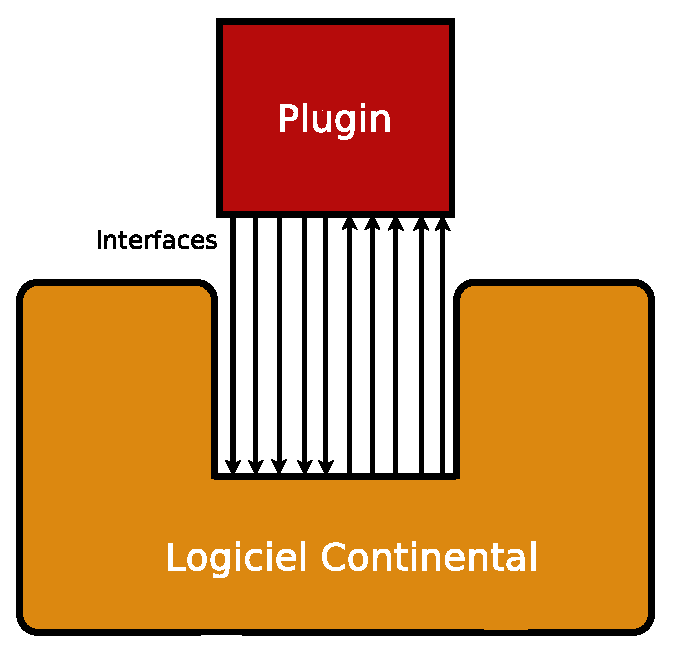
\includegraphics[width=3cm]{images/plugin.eps}
		\caption{\scriptsize Intégration du \textit{plugin}}
		\end{figure}		
	\end{wrapfigure}

	\vfill
	\vspace{-10px}
	\begin{minipage}{0.6\textwidth}
			Intégration du << plugin >>
			\begin{itemize}
				\item Fourni par le client
				\item Doit s'interfacer avec les logiciels Continental 
				\item Spécification des variables fournie au format Excel
			\end{itemize}
				\end{minipage}
			\pause
	\vfill	
	\vspace{20px}
	\begin{alertblock}{Difficile à tester}
		Tests manuels qui sont : 
		\begin{itemize}
			\item Non exhaustifs
			\item Longs à faire
			\item Répétitifs
		\end{itemize}
	\end{alertblock}
	\vfill
\end{frame}

